%%
%% This is file `sample-sigchi.tex',
%% generated with the docstrip utility.
%%
%% The original source files were:
%%
%% samples.dtx  (with options: `sigchi')
%% 
%% IMPORTANT NOTICE:
%% 
%% For the copyright see the source file.
%% 
%% Any modified versions of this file must be renamed
%% with new filenames distinct from sample-sigchi.tex.
%% 
%% For distribution of the original source see the terms
%% for copying and modification in the file samples.dtx.
%% 
%% This generated file may be distributed as long as the
%% original source files, as listed above, are part of the
%% same distribution. (The sources need not necessarily be
%% in the same archive or directory.)
%%
%% The first command in your LaTeX source must be the \documentclass command.
\documentclass[sigplan]{acmart}
\usepackage{booktabs}
\usepackage{todonotes}
%%
%% \BibTeX command to typeset BibTeX logo in the docs
\AtBeginDocument{%
  \providecommand\BibTeX{{%
    \normalfont B\kern-0.5em{\scshape i\kern-0.25em b}\kern-0.8em\TeX}}}

%% Rights management information.  This information is sent to you
%% when you complete the rights form.  These commands have SAMPLE
%% values in them; it is your responsibility as an author to replace
%% the commands and values with those provided to you when you
%% complete the rights form.
\setcopyright{acmcopyright}
\copyrightyear{2018}
\acmYear{2018}
\acmDOI{10.1145/1122445.1122456}

%% These commands are for a PROCEEDINGS abstract or paper.
\acmConference[Woodstock '18]{Woodstock '18: ACM Symposium on Neural
  Gaze Detection}{June 03--05, 2018}{Woodstock, NY}
\acmBooktitle{Woodstock '18: ACM Symposium on Neural Gaze Detection,
  June 03--05, 2018, Woodstock, NY}
\acmPrice{15.00}
\acmISBN{978-1-4503-XXXX-X/18/06}


%%
%% Submission ID.
%% Use this when submitting an article to a sponsored event. You'll
%% receive a unique submission ID from the organizers
%% of the event, and this ID should be used as the parameter to this command.
%%\acmSubmissionID{123-A56-BU3}

%%
%% The majority of ACM publications use numbered citations and
%% references.  The command \citestyle{authoryear} switches to the
%% "author year" style.
%%
%% If you are preparing content for an event
%% sponsored by ACM SIGGRAPH, you must use the "author year" style of
%% citations and references.
%% Uncommenting
%% the next command will enable that style.
%%\citestyle{acmauthoryear}

\newcommand{\theArticle}{\textit{Towards innovation measurement in the software industry}}
%%
%% end of the preamble, start of the body of the document source.
\begin{document}

%%
%% The "title" command has an optional parameter,
%% allowing the author to define a "short title" to be used in page headers.
\title{The Impact of a Proposal for Innovation Measurement in the Software Industry}

%%
%% The "author" command and its associated commands are used to define
%% the authors and their affiliations.
%% Of note is the shared affiliation of the first two authors, and the
%% "authornote" and "authornotemark" commands
%% used to denote shared contribution to the research.
\author{Nauman bin Ali}
\orcid{0000-0001-7266-5632}
\affiliation{%
  \institution{Blekinge Institute of Technology}
  \country{Sweden}}
\email{nal@bth.se}

\author{Henry Edison}
\affiliation{%
  \institution{Lero, NUI Galway}
  \country{Ireland}}
\email{henry.edison@nuigalway.ie}

\author{Richard Torkar}
 \orcid{0000-0002-0118-8143}
 \affiliation{
 \institution{Chalmers and University of Gothenburg}
 \country{Sweden}
 }
 \affiliation{
 \institution{Stellenbosch Institute for Advanced Study (STIAS)}
 \country{South Africa}
 }
 \email{torkarr@chalmers.se}


%%
%% By default, the full list of authors will be used in the page
%% headers. Often, this list is too long, and will overlap
%% other information printed in the page headers. This command allows
%% the author to define a more concise list
%% of authors' names for this purpose.
\renewcommand{\shortauthors}{Ali et al.}

%%
%% The abstract is a short summary of the work to be presented in the
%% article.



\begin{abstract}
Measuring an organization's capability to innovate and assessing its innovation output and performance on the market is a challenging task. We proposed a comprehensive model and a suite of measurements to support this task. In the current paper, we have reflected on the impact of the work. We have mainly relied on quantitative and qualitative analysis of the citations of the paper.  
\end{abstract}

%%
%% The code below is generated by the tool at http://dl.acm.org/ccs.cfm.
%% Please copy and paste the code instead of the example below.
%%
\begin{CCSXML}
<ccs2012>
 <concept>
  <concept_id>10010520.10010553.10010562</concept_id>
  <concept_desc>Computer systems organization~Embedded systems</concept_desc>
  <concept_significance>500</concept_significance>
 </concept>
 <concept>
  <concept_id>10010520.10010575.10010755</concept_id>
  <concept_desc>Computer systems organization~Redundancy</concept_desc>
  <concept_significance>300</concept_significance>
 </concept>
 <concept>
  <concept_id>10010520.10010553.10010554</concept_id>
  <concept_desc>Computer systems organization~Robotics</concept_desc>
  <concept_significance>100</concept_significance>
 </concept>
 <concept>
  <concept_id>10003033.10003083.10003095</concept_id>
  <concept_desc>Networks~Network reliability</concept_desc>
  <concept_significance>100</concept_significance>
 </concept>
</ccs2012>
\end{CCSXML}

\ccsdesc[500]{Computer systems organization~Embedded systems}
\ccsdesc[300]{Computer systems organization~Redundancy}
\ccsdesc{Computer systems organization~Robotics}
\ccsdesc[100]{Networks~Network reliability}

%%
%% Keywords. The author(s) should pick words that accurately describe
%% the work being presented. Separate the keywords with commas.
\keywords{innovation, impact, relevance, measurement}


%%
%% This command processes the author and affiliation and title
%% information and builds the first part of the formatted document.
\maketitle


\section{Introduction}\label{sec:intro}\todo {Richard}
Innovation measurement in SE was a challenge---we contributed with a measurement framework in \theArticle~\cite{EdisonAT13}. 

The paper is structured as follows: Section \ref{sec:sumpaper} summarizes the contribution of \theArticle. In Section \ref{sec:whocites}, we describe a content analysis of the articles citing \theArticle. Section \ref{sec:soa} discusses the research identified in Section \ref{sec:whocites} that has extended our work. In Section \ref{sec:impact}, we discuss the research which documents the use of our work in industrial settings. Section \ref{sec:fw} concludes the paper with some suggested directions for future research.

\section{Summary and main contributions of \theArticle}
\label{sec:sumpaper}
Over the past, companies relied on cost and lead time reduction and quality improvement to strengthening their competitiveness. While quality is necessity, today it is not sufficient. Companies must continuously innovate; develop new processes and deliver new products to achieve and sustain a competitive advantage. Otherwise, they tend to lose their position to new and emerging startups that have innovative offerings. Such turnover signifies the importance of sustained innovation, thus the problem is not happen-stance innovation but rather doing it continuously on a regular basis. For sustained innovation to become a reality, a better understanding of innovation is required, which is possible only when innovation is measured.

The important of innovation measurement is well emphasised in industry. The Boston Consulting Group's survey \cite{andrew08} revealed that most executives believe that their companies should measure innovation as rigorously as core business operation, but less than half of companies actually do so. There is little consensus on how innovation measurement should be carried out. Each definition of innovation that is used signify a different aspect of innovation, e.g. perspectives, levels and types etc. This in turn determines what is considered as elements of innovation and how these are measured.

Organisations require means not only to measure their innovative output but also to assess their ability and capacity to innovate. Measurement helps to better understand and evaluate the consequences of the initiatives geared towards innovation. Furthermore,  like any other measurements, these will allow organisations to specify realistic targets of innovation in the future and to identify and resolve problems hindering progress towards goals, making. decisions and continuously improve the abilities to innovate.

The aims of this study were to establish the state of the art of innovation measurement and to capture the state of the practice of innovation measurement in the software industry. A systematic literature review (SLR) \cite{kitchenham07}  was conducted to establish the state of the art of innovation measurement, followed by a web-based questionnaire \cite{kasunic05} and face-to-face interviews \cite{creswell09} to collect the opinions of software industry practitioners and academics. In total, we retrieved 13,401 articles from seven digital libraries (Compendex, Scopus, IEEEXplore, ACM Digital Library, ScienceDirect and Business Source Premiere). After applying inclusion/exclusion criteria, 204 papers were accepted as the primary studies. We had 145 respondents out of which 94 completed the questionnaire - thus the completion rate was 54.83\%. Four industry practitioners (middle managers) and three academics with close relationship with industry were interviewed in this study. 

Our review shows that there are 41 definitions of innovation found in the literature which highlight 4 important attributes to measure: 
\begin{itemize}
	\item Impact of innovation on the market and technology, e.g. incremental or radical innovation, market or technological breakthrough.
	\item Types of innovation, e.g. product (new or significantly improved products), process (new or significantly improved design, analysis, or development method), market (new or significantly improved marketing methods, strategies, and concept in product design or packaging, placement, promotion, or pricing), and organisation innovation (new or significantly improved organisation methods, e.g. business practices, workplace organisation or external relations.
	\item Degree of novelty, e.g. new to the firm, new to the market, new to the world, and new to the industry.
	\item Nature of process: iterative process.
\end{itemize}

While twenty-eight determinants of innovation have been reported in literature, but only seven of them are studied in the software industry: internal collaboration, customer orientation, champions, human resources, strategy, networking, and leadership. Two-hundred and thirty-two metrics have been used to measure innovation in firm (88\%), industry (1\%), regional level (11\%). However, only 37\% of them have been statistically validated and 58\% have never been used in practice. Our review also identifies 13 innovation measurement frameworks. Most of these framework focus on technological breakthrough (8 frameworks). Out of these frameworks, only one framework have been studied in software companies. 

The results of the interview and the questionnaire are consistent with the view of the impact, types and the dimension of novelty of innovation. The experts and respondents with management and executive roles perceive innovation at a much broader level and emphasise the market and organisation innovations by using abstract concepts like value creation and need fulfilment. They looked at the purpose and goal to define what may be considered as innovation. While respondents with technical roles have a strong inclination on product innovation as they mainly involved in product development.

There is also an agreement on the importance of innovation measurement from the interviews and the questionnaire results but the practice is still lagging behind. Majority of respondents and experts reported the lack of explicit innovation strategy and measurement programme. Moreover, innovation measurement suffers from the following challenges:
\begin{itemize}
	\item Lack of consistent definition of innovation. Definitions are fundamental as they affect the measurement program and help provide a common understanding.
	\item Lack of meaningful metrics. For example, R\&D measures (e.g. percentage of sales spent on R\&D, number of R\&D staff, etc) only focus on input and may not be applicable in small and medium enterprises. Similarly, the IPR-based measures (e.g. patent counts, and citation-based data, etc) may no represent innovation at all - prevent competitor from exploiting opportunities.
	\item Lack of frameworks to guide innovation measurement. Measurement frameworks. consist of a set of related metrics, data collection mechanism and. data uses inside a company. However, as there is no clear understanding what innovation us, there is also no agreement on what metrics should be collected.
\end{itemize}

Using the different perspectives of innovation and the key aspects for innovation measurement as identified by the systematic literature review, we developed an innovation measurement model, as shown in Fig. \ref{ig:im_model}. This model was further refined after preliminary evaluation by academics and practitioners. From the outset, the model identifies three main elements of measurement: innovation capability, innovation output and impact of innovation. Unlike the current strict reliance on sales as the sole measure for innovation, which may produce negative effects on the innovation climate of the organisation, this model highlights the opportunity of a more comprehensive approach towards innovation measurement. Each of these aspects identified in the model can be measured quantitatively (using both objective and subjective metrics). Metrics for each of these aspects identified from literature have been aggregated and categorised in this study.

\begin{figure*}[!ht]
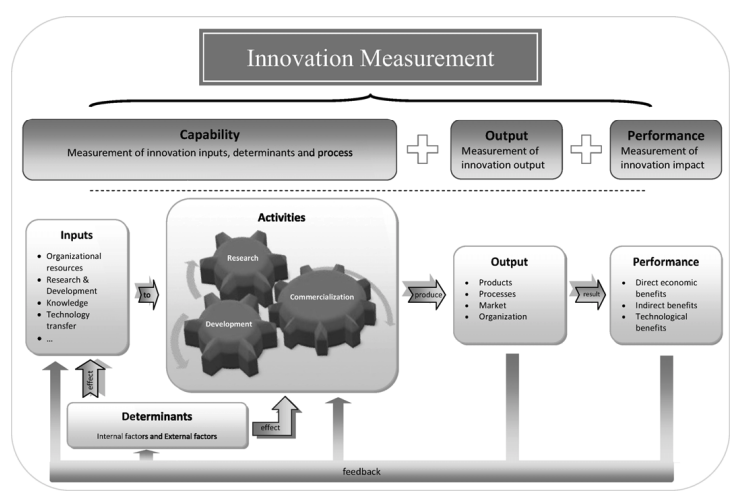
\includegraphics[width=0.8\textwidth]{Figures/im_model}
\caption{Innovation Measurement Model}
\label{fig:im_model}
\end{figure*}

In terms of implications, the paper makes three contributions to both research and practice. First, this study aggregated the available empirical evidence reported in literature to establish the state of the art in innovation measurement through an extensive literature review. The outcome of this review contributed to the existing body of knowledge in the form of an innovation measurement model, enumeration of metrics and their classification based on what aspect of innovation they are used to measure. The second contribution is to provide an innovation measurement model, which is founded in empirical research and has been evaluated by experts. The model captures various dimension of innovation. Industry practitioners could use our findings to reflect on their experience on innovation measurement in order to minimise the challenges in their contexts. Finally, the study provides future direction for innovation measurement research.



\section{Methodology}\label{sec:method} \todo{Nauman}
For understanding the impact of \theArticle, we have relied on the classification schema for academic citations proposed by \citet{teufel2006annotation}. We also considered the taxonomy proposed by \citet{bornmann2008citation}. However, based on a pilot application we found \citet{teufel2006annotation} more straight forward and sufficient for our analysis. The decision is further supported by prior experience of using Bornmann and Daniel's taxonomy in software engineering literature \cite{poulding2015using}.

The categories in the schema we used are listed and briefly described in Table~\ref{tab:CitationCategories}. To separate any industrial application of our work we added a separate category. 

On February 24, 2020, the \theArticle  had over 72 citations in Science Direct and Scopus, 61 in Web of Science Core Collection, and 234 in Google Scholar. To get a relatively complete picture of how this work has impacted further research, we decided to analyse the 234 citations on Google Scholar. 

In a pilot, the first two authors classified ten randomly selected articles and discussed the use of categories. Thereafter, they divided the 234 articles among them and  independently classified them. The procedure followed is briefly summarized below: 
\begin{itemize}
\item Exclude citations where the full-text is not available. 
\item Exclude articles which are not written in English.
\item Exclude articles  that do not cite \theArticle in the full-text.
\item From the title, abstract and the publication venue judge the discipline of the publication (e.g. software industry, manufacturing, farming or automotive).
\item Only for conference papers and journal article, search for the citation to \theArticle in the full text, for each citation in the paper  read the entire paragraph containing it to understand the context, then classify the citation based on categories in Table \ref{tab:CitationCategories}.
\end{itemize}
 


\begin{table*}
	\caption{Categories of citing papers from \citet{teufel2006annotation}}\label{tab:CitationCategories}
	\begin{tabular}{llp{12cm}}
		\toprule
		\textbf{Category}            & \textbf{Sub-category }& \textbf{Description}                                                                                                            \\ \midrule
		Weakness            & Weak         & Weakness of the approach pursued in \theArticle, Weakness in the definition, model, entities, attributes, or measurements of innovation as proposed in \theArticle                                                                                              \\
		\midrule
		Contrast/Comparison & CoCoGM       & Contrast/Comparison in Goals or Methods (neutral)                                                                    \\
		& CoCoR0       & Contrast/Comparison in Results (neutral)                                                                               \\
		& CoCo-        & Unfavourable Contrast/Comparison (current work is better than the work in \theArticle)                                            \\
		& CoCoXY       & Contrast between a cited method and the method in \theArticle                                                                                     \\
		
		\midrule
		Positive sentiment  & PBas         & author uses the work in \theArticle as a starting point                                                                               \\
		& PUse         & author uses definitions/models/measures                                                                                      \\
		& PIUse\footnote{We have added this category}         & author uses the work in \theArticle in industrial settings \\
		& PModi        & author adapts or modifies definition/model/measurements  presented in \theArticle                                                                            \\
		& PMot         & this citation is positive about approach or problem addressed in \theArticle (used to motivate work in current paper)                 \\
		& PSim         & author’s work and the work in \theArticle are similar                                                                               \\
		& PSup         & author’s work and the work in \theArticle are compatible/provide support for each other                                           \\
		
		\midrule
		Neutral             & Neut         & Neutral description of cited work, or not enough textual evidence for above categories.\\
		\bottomrule
	\end{tabular}
\end{table*}

\section{Overview of the papers citing \theArticle}\label{sec:whocites} \todo{Nauman} %covers: Who found it relevant (would be good to have some qualitative data on how they ref the paper). Why did so many cite it?}

The 234 citations to\theArticle were analysed using the process described in the Section \ref{sec:method}. Figure~\ref{fig:selection} provides the results of the selection steps. In total 118 citations were excluded from further analysis. 54 were considered grey-literature i.e. books, technical reports and theses. A majority i.e. 42 of the 54 citations in the grey-literature were masters or doctoral theses. Similarly the remaining 64 of the 118 citations were excluded for other reasons (language of the publication, inaccessible full-text, incorrect citation and duplicate citations). A clear majority 52 of the 64 citations excluded in this group were not read in full-text as they were not written in English.

Two interesting results emerge from this data: (1) that a significant number of publications not written in English have cited \theArticle, and (2) almost an equal number of citations are from grey literature. This indicates that systematic literature reviews in software engineering, like in medicine, should also develop a strategy to consider such literature or at the least consider the impact of not including such literature in SLRs.

\begin{figure}[htbp]
	\begin{center}
		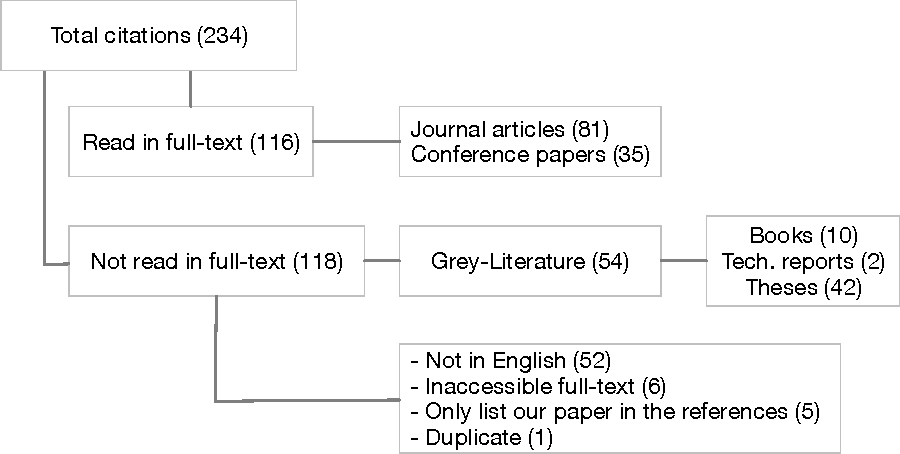
\includegraphics[width=0.45\textwidth,height=\textheight,keepaspectratio]{Figures/Citations.pdf}
	\end{center}
	\caption{Results of applying selection criteria on the citations}
	\label{fig:selection}
\end{figure}

%Exclude papers 64 (52  were not written in English, 6 were inaccessible in full-text, 5 did not cite \theArticle in the body of the paper and 1 was a duplicate citation).
%Grey literature:  53 citations are from what we have classified as grey  literature. Of these 53, 2 are  technical reports, 10 are book chapters and 41 are theses.

The remaining 116 of the 234 citing papers were read in full-text. Of these 81 are journal articles and 35 are conference papers citing \theArticle. This is an interesting result in itself as \theArticle is getting significantly more citations from journal articles and grey-literature than conference papers. When looking at the publication forums from software engineering and other fields we see a different pattern. In SE, 24 of the 44 (55\%) citing papers are journal articles and remaining 20 (i.e. 45\%) are conference papers. Where as in the 72 citing articles from other fields 57 (i.e. 80\%) are journal articles and 15 (i.e. 20\%) are conference papers. We speculate that this may be an artifact of different traditions of publications in different fields i.e. other fields may not have similar tradition of conference proceedings or even a similar frequency of conferences.


The analysis of the use of \theArticle in 116 conference papers and journal articles is summarized in Table \ref{tab:CitationAnalysis}. Only eight self citations were identified. 

In \theArticle, we proposed a model and metrics based on a consolidation of research from other fields for software development field. However, it is interesting to observe that the article has been cited frequently in literature from outside software engineering. Only 44 of the 116 (i.e. 38\%) of the publications are on topics related to software development. A majority, 67 of the 116 (i.e. 62\%) of the citing articles have no stated connection to the context of the software industry. These articles encompass several diverse fields including the following: automotive, banking, economics, farming, forestry, health sector, human resources, logistics, manufacturing, mechatronics, NGOs, oil industry, politics, restaurants and transportation.  A more detailed analysis of the reasons for the citations will help speculate the reason for this disparity.

Overall, in terms of the categories of the citing article (please see Table \ref{tab:CitationCategories} for a listing and the definitions of the categories) 75 of 116 (i.e. 65\%) are neutral, 38 of 116 (i.e. 32\%) are neutral, and only 2 of 116 (i.e. less than 1\%) present a comparison/contrast. Surprisingly, we did not find any papers identifying or discussing a weakness of the research documented in \theArticle.
 
We expected that the number of citing articles in different categories will be different for literature from software engineering research and other fields. As we expected more citations identifying weaknesses, presenting comparisons and building on our work from within our discipline. However, similar patterns of citation appear both in and outside software engineering. In software engineering literature, of the 44 citing papers, 17 (i.e. 39\%) are positive, 27 (i.e. 61\%) are neutral while no comparison/contrast or weaknesses of \theArticle are presented. Among the 72 citing papers from other fields, 21 (i.e. 29\%) are positive, 48 (i.e. 67\%) are neutral while 2 citing papers present a comparison/contrast and no citing papers present any weaknesses of \theArticle. Therefore, no discernible difference in citing categories are observed. 

A majority i.e. in 21 of the 38 ( 55\%) citing articles with in the "positive" category, use the definition, metrics or the model proposed in \theArticle. The next most frequent (12 of the 38 cases in the category i.e. 32\%) positive use of \theArticle is as a starting point or motivation for their work. A few articles also describe that they adapted the definitions presented in \theArticle or considered their work similar or supporting the work presented in \theArticle. 

However, we found no documented evidence of applying the model or metrics given in \theArticle in industry in the citing papers. Perhaps they grey literature not considered for the detailed analysis in this study may have reported such a case as an experience report or technical report.



\begin{table*}
	\caption{Results of an analysis of the citing papers}
	\label{tab:CitationAnalysis}
	\begin{tabular}{p{2.5cm}llp{1.5cm}llll}
			\toprule
		& Total & Weak & Comparison / Contrast & Positive                                            & Neutral & Jrnl. & Conf. \\
		\midrule
		&       &      &                       &                                                     &         &         &            \\
		Self citations               & 8     & 0    & 0                     & 2 (PBas:1, PMot:1, PModi:1)                         & 6       & 5       & 1          \\
		From software related fields & 44    & 0    & 0                     & 17 (PBas:4, PModi:2,PUse:7,PMoti:4, PSup:1)         & 27      & 24      & 20         \\
		Others                       & 72    & 0    & 2                     & 21 (PBas:2, PModi:2,PUse:14,PMoti:2,PSim:1, PSup:2) & 48      & 57      & 15         \\
		Total                        & 116   & 0    & 2                     & 38 (PBas:6, PModi:2,PUse:21,PMoti:6,PSim:1, PSup:3) & 75      & 81      & 35        \\ \bottomrule
	\end{tabular}
\end{table*}

While discussing the citations the following reference will be useful \cite{penders2018ten} We can use this to also articulate why we have relied on citations as a way to reflect on the paper.


\section{Positioning in consideration of the recent state of the art and practice}\label{sec:soa} \todo{Henry}
What has been done after this (partly we'll get it from the previous section).
Open innovation seems to be the area in SE that has been a follow-up of our work.

\section{Expected impact}\label{sec:impact}
Here it would be nice to show cases in industry not counting Ericsson. Perhaps we can get it from Section~\ref{sec:whocites}?



\section{New emerging ideas and current vision}\label{sec:fw} \todo{Possibly Richard?}
What will be done, possibly

\section*{Acknowledgement}
This project has received funding from the European Union's Horizon 2020 research and innovation programme under the Marie Skłodowska-Curie grant agreement No. 754489 and with the financial support of the Science Foundation Ireland grant 13/RC/2094. This work has been supported by ELLIIT, a Strategic Area within IT and Mobile Communications, funded by the Swedish Government. The work has also been supported by research grants for the VITS project (reference number 20180127) from the Knowledge Foundation in Sweden.

%\section*{References}

%%
%% The acknowledgments section is defined using the "acks" environment
%% (and NOT an unnumbered section). This ensures the proper
%% identification of the section in the article metadata, and the
%% consistent spelling of the heading.
%\begin{acks}
%\end{acks}



%%
%% The next two lines define the bibliography style to be used, and
%% the bibliography file.
\bibliographystyle{ACM-Reference-Format}
\bibliography{sample-base}

%%
%% If your work has an appendix, this is the place to put it.
%\appendix

%\section{Research Methods}


\end{document}
\endinput
%%
%% End of file `sample-sigchi.tex'.
%There are some more interesting ideas for inspiration in the CFP for SANER https://saner2020.csd.uwo.ca/eratrack